\documentclass[12pt,onecolumn]{biophys}
%\documentclass[12pt,twocolumn]{article}
%\documentclass[twocolumn]{biophys}
\usepackage{amssymb,amsfonts,amsthm,bm}
\usepackage[round,numbers,sort&compress]{natbib}
\usepackage[ansinew]{inputenc}
\gridframe{N}

\usepackage{amssymb,amsfonts,amsthm,bm}
\usepackage[round,numbers,sort&compress]{natbib}
\usepackage{graphicx}
\usepackage{amssymb}
\usepackage{fixltx2e}
\usepackage{graphicx}
\usepackage{wrapfig, blindtext}
\usepackage{setspace} 
\usepackage{caption}
\usepackage{subcaption}
\usepackage{subfig}
\usepackage[ansinew]{inputenc}

\begin{document}
\newcommand{\WT}{Wild-type\xspace}
\newcommand{\MT}{Mutant\xspace}
\newcommand{\RMSD}{RMSD(symm)\xspace}
\newcommand{\WTs}{Wild-types\xspace}
\newcommand{\MTs}{Mutants\xspace}
\newcommand{\RMSDs}{RMSDs(symm)}
\renewcommand{\thefigure}{S\arabic{figure}}
\setcounter{figure}{0}




\begin{figure}
\begin{center}
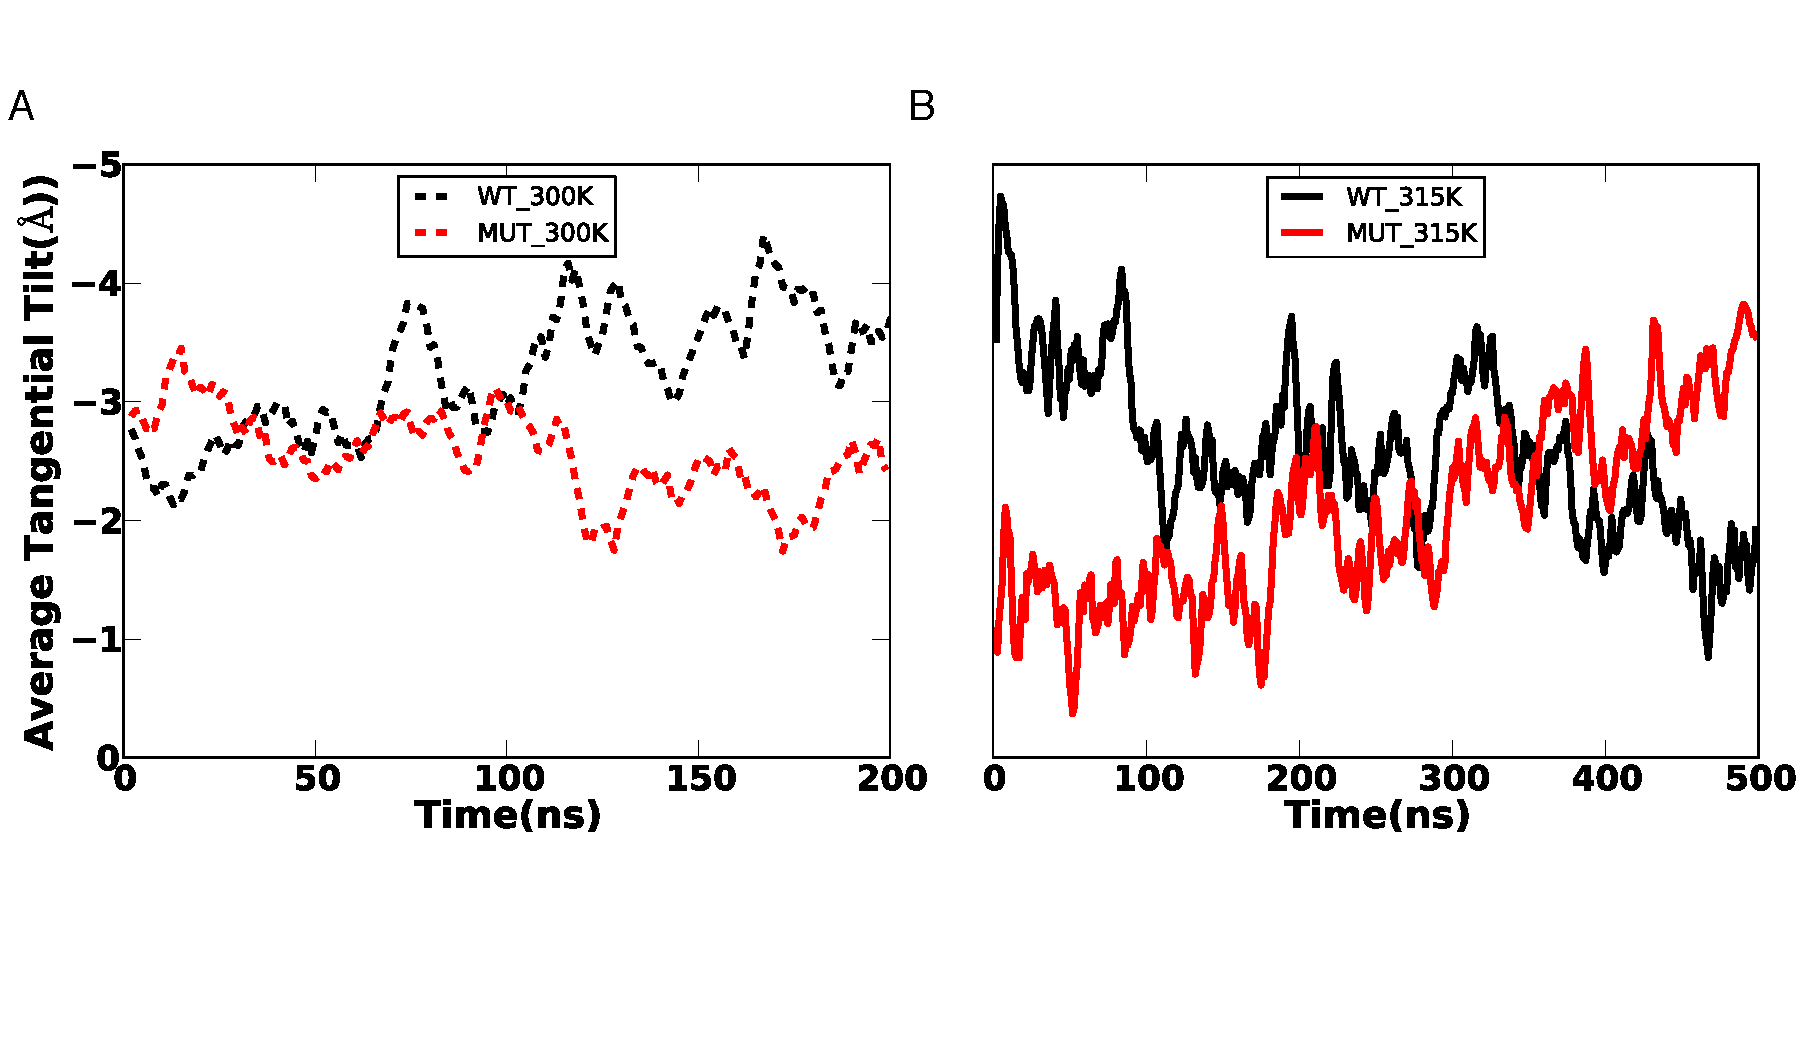
\includegraphics[width = 1\textwidth]{figures/Sup-tangential_tilt.pdf}
\end{center}
\caption{Average Tangential Tilt of the M2 helices (A) at 300K and (B). at 315K.}
\label{fig:avgTilt}
\end{figure}




\begin{figure}
\begin{center}
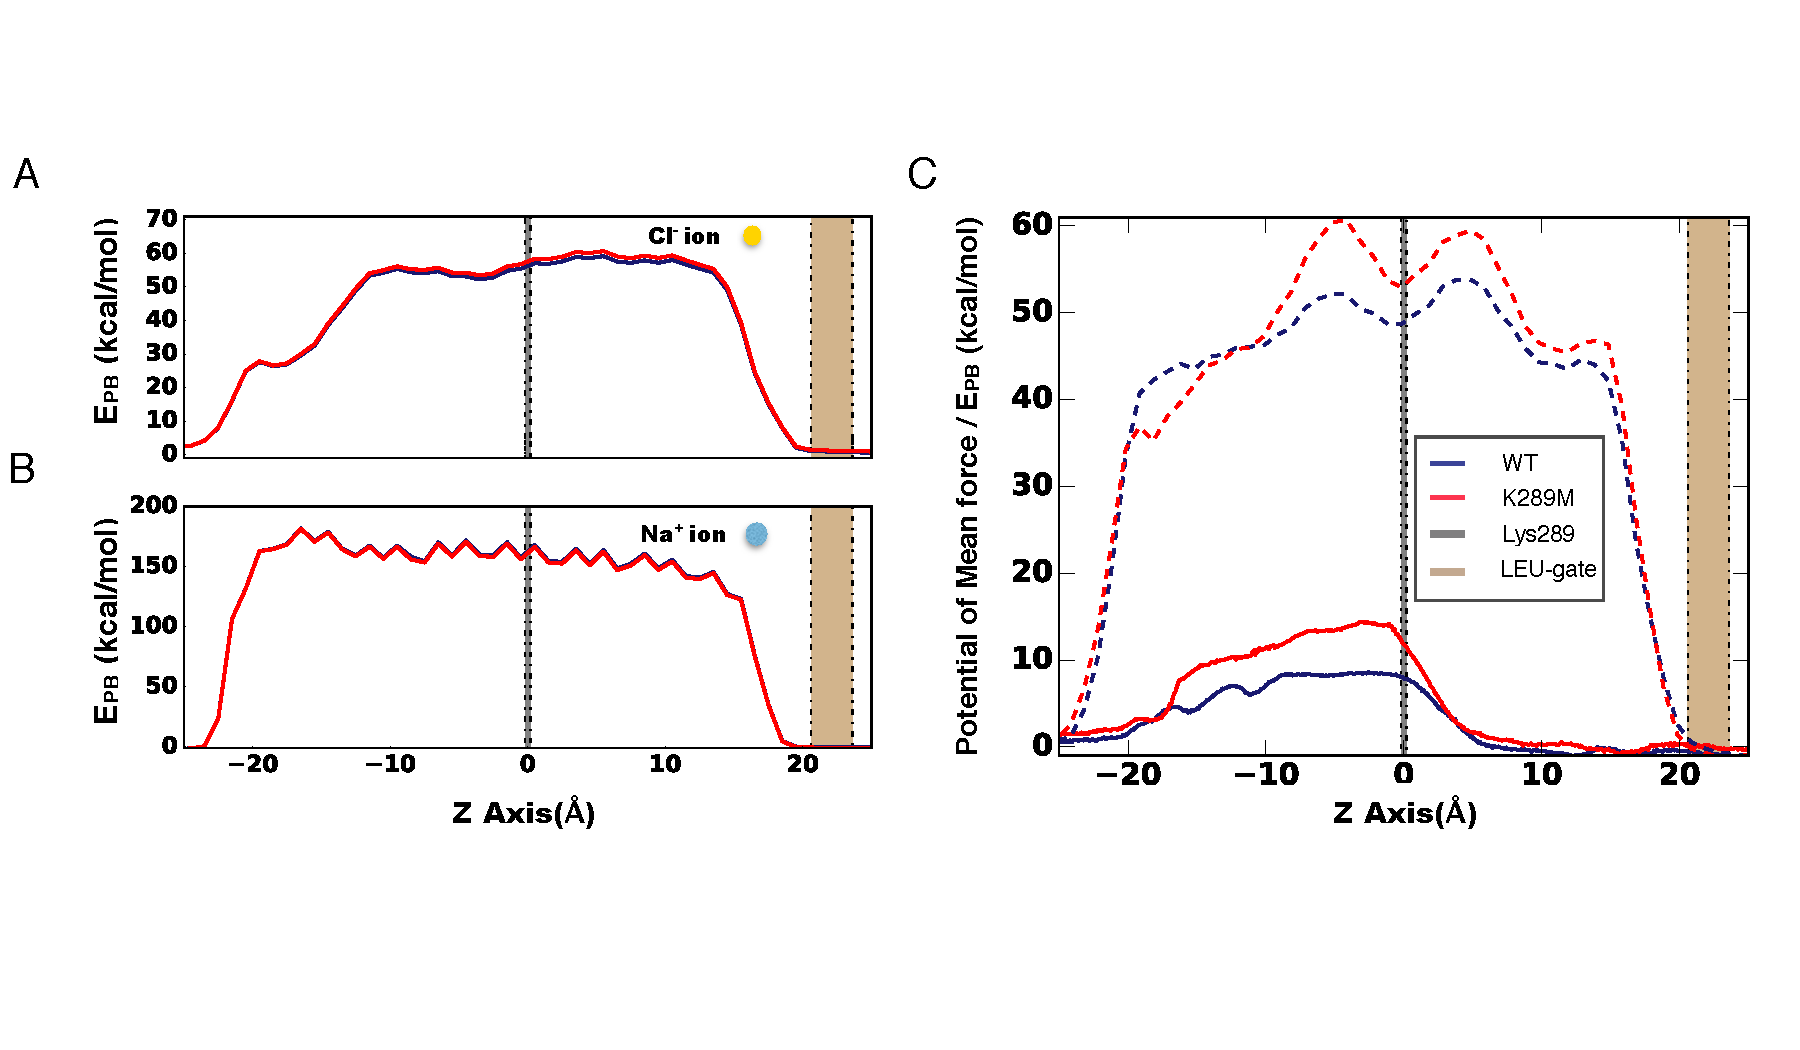
\includegraphics[width = 1\textwidth]{figures/sup2_APBS}
\end{center}
\caption{Poisson-Boltzmann profile: (A)Electrostatic environment in the initial configuration of the channel as experienced by a chloride(top) and sodium(bottom) ion, calculated by performing a Poisson?Boltzmann profile along the TMD. (B)Average of the electrostatic barriers over the final 50ns of the simulation at lower(300K) and higher(315K) temperature.(C)Plot compares the electrostatic barriers from the PB profile to the PMF calculated using ABF simulations.}
\label{fig:APBS_2}
\end{figure}

%\begin{figure}
%\begin{center}
%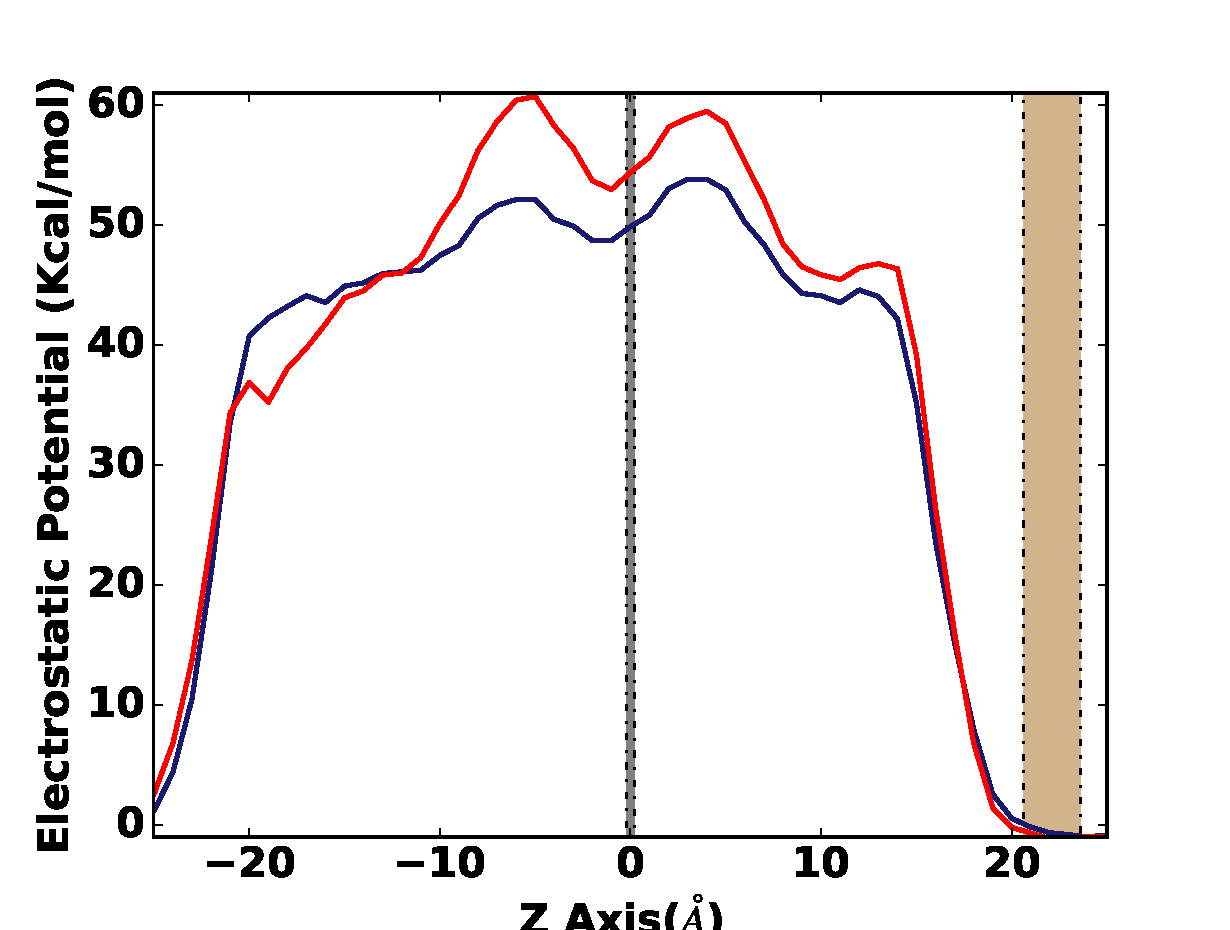
\includegraphics[width = 100mm]{figures/APBS_COMP.pdf}
%\end{center}
%\caption{The Electrostatic potential profiles along the channel pore (for a chloride ion - averaged over 50ns) for the higher  temperature systems. Implicit solvent calculations, performed using APBSmem provided indication about possible barriers in the channel and also the significant difference between the \WT and the \MT.}
%\label{fig:apbs}
%\end{figure}

\begin{figure}
\begin{center}
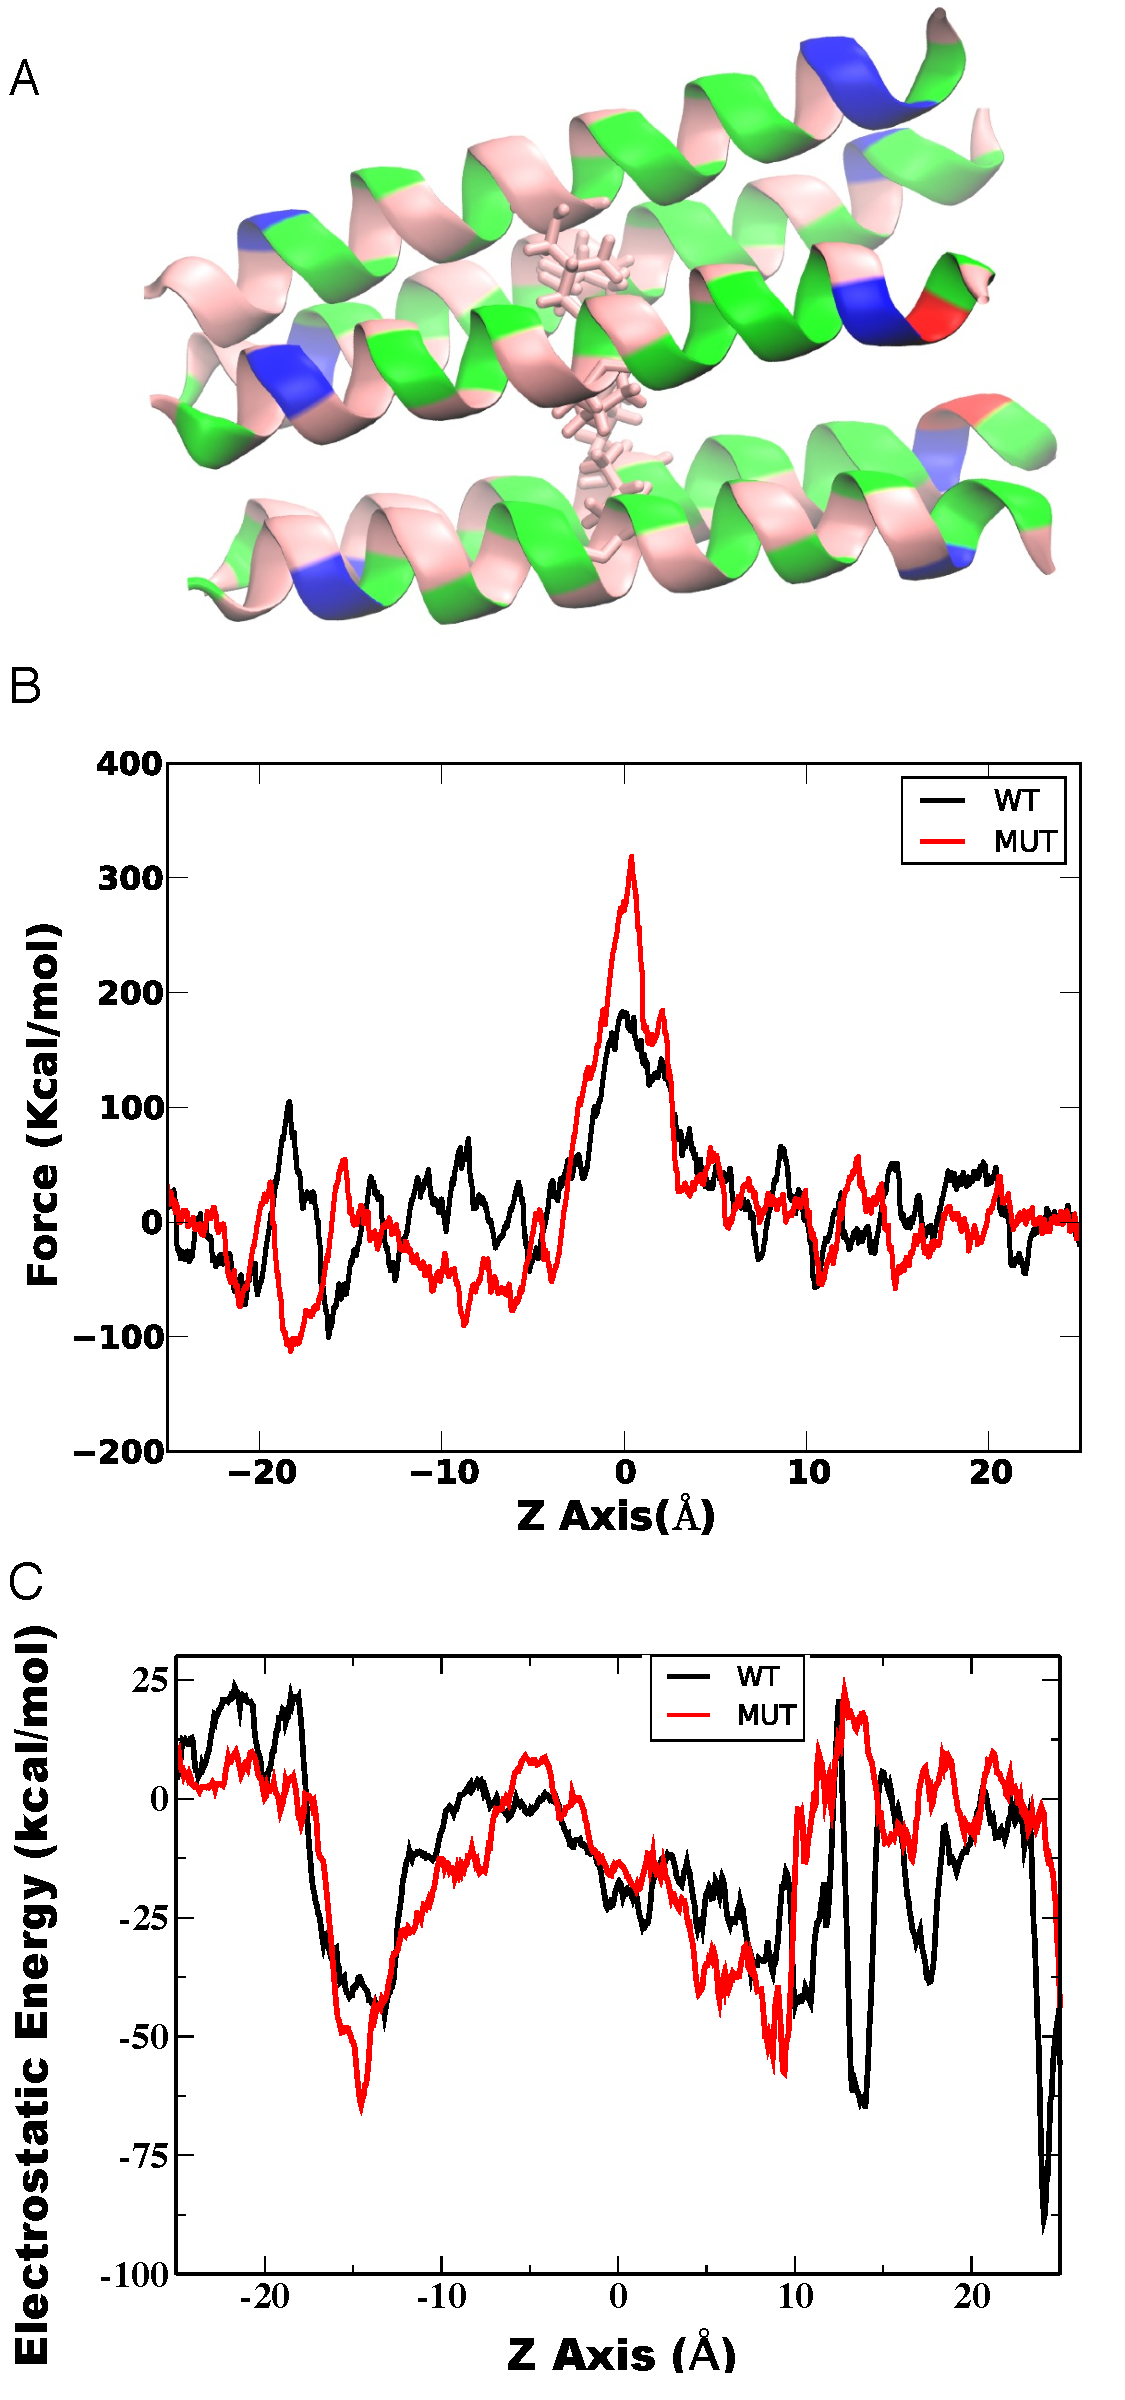
\includegraphics[width = 80mm]{figures/sup1_SMD}
\end{center}
\caption{(A) Snap-shot depicting the M2-helices (laid horizontally) showing the minimum constriction region flanked by LEU residues.(B) The force experienced by the ion as a function of position in the channel along the Z axis(TM domain).(C) Electrostatic effects of protein on the chloride moving through the channel.}
\label{fig:SMD}
\end{figure}



\begin{figure}
\begin{center}
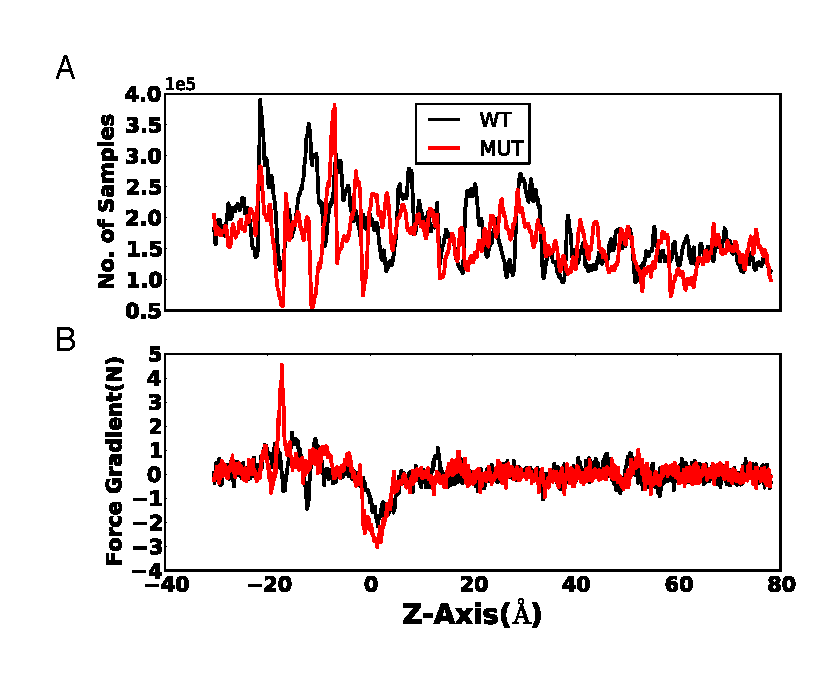
\includegraphics[width = 100mm]{figures/Sup_ABF_plots_comp.pdf}
\end{center}
\caption{(A) Number of samples generated in each window of the ABF run. (B) Gradient of the force experienced by the ion in each window of the ABF run. }
\label{fig:ABF_2}
\end{figure}

\end{document}